\documentclass[10pt,a4paper]{article}
\usepackage[margin=2.2cm]{geometry}
\usepackage{fontspec}
\usepackage{amsmath,amssymb}
\usepackage{booktabs,graphicx,float,xcolor,array}
\usepackage[font=small,labelfont=bf]{caption}
\usepackage{enumitem}
\usepackage[colorlinks=true,linkcolor=blue!50!black,urlcolor=blue!50!black,citecolor=blue!50!black]{hyperref}
\setlist{itemsep=2pt,topsep=3pt}
\graphicspath{{../figures/round2/}}
\newcommand{\tabin}[1]{\IfFileExists{tables_r2/#1.tex}{\input{tables_r2/#1.tex}}{}}
\newcommand{\code}[1]{\texttt{#1}}

\title{\textbf{Scaling NBN, round 2: the other mechanisms and inference engines}\\[4pt]
\large kNN, FlexCode, neural categorical, normalising flows, amortized IS and VI, certified routing}
\author{Alfredo (\code{alfredo\_claude}) for Giovanni Briglia}
\date{17 October 2026 --- branch \code{feat/scaling-mechanisms} (on top of \code{feat/scaling-study}), local, not pushed}

\begin{document}
\maketitle

\section*{Summary}
The first round sped up exact inference, likelihood weighting, MDN fitting and the S4 set
builders. This round applies the same rule (\emph{faster, with the same answers}) to the rest of
NBN: the neural categorical, FlexCode and flow mechanisms, the kNN mechanism, amortized importance
sampling, amortized variational inference, and the inference router. Every change was planned with
the \code{koller\_claude} and \code{moss\_claude} experts (Koller \& Friedman; Algorithms for
Validation), is covered by an equivalence test, and is benchmarked under the same budget as round 1
(1 CPU thread, 4\,GB, 30\,s). Each change is compared with NBN \code{master}, with the first
scaling branch, and with pgmpy or Pyro where an equivalent exists. pgmpy has no neural,
kNN or flow CPDs and no amortized engines, so it is a baseline only in round 1.

\begin{figure}[H]\centering
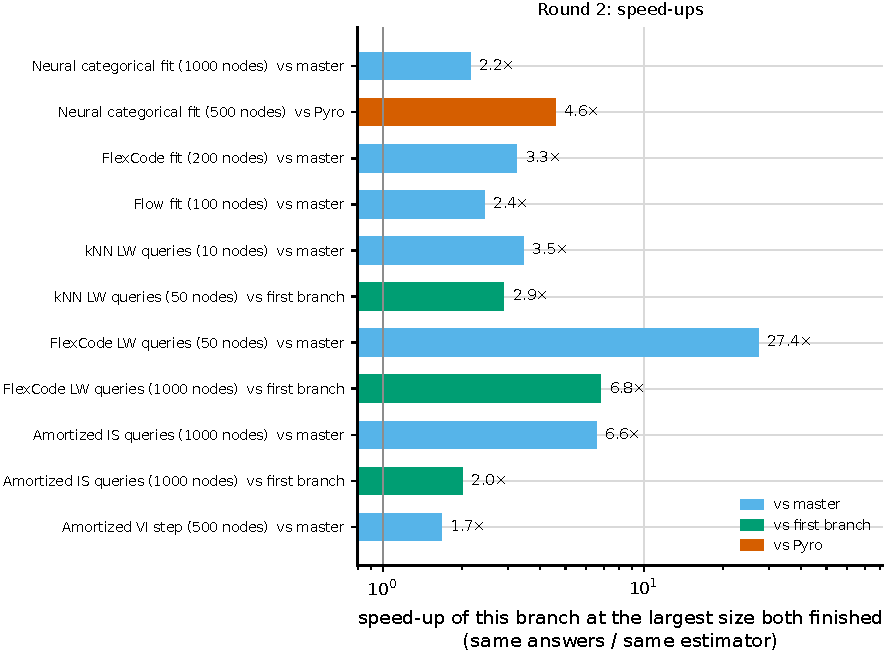
\includegraphics[width=0.85\linewidth]{r2_0_summary.pdf}
\caption{Speed-ups of this branch at a representative size.}
\end{figure}
\tabin{r2sum}

\section{What changed, and why the answers stay the same}
\begin{table}[H]\centering\small
\caption{Changes of round 2 (7 commits; full unit and integration suites green).}
\resizebox{\linewidth}{!}{%
\renewcommand{\arraystretch}{1.15}\begin{tabular}{>{\raggedright\arraybackslash}p{0.22\linewidth}>{\raggedright\arraybackslash}p{0.32\linewidth}>{\raggedright\arraybackslash}p{0.40\linewidth}}\toprule
change & what it does & why the answers do not change \\ \midrule
Stacked fitting for neural categorical, FlexCode and flows (\code{fit(method="stacked")}) & one batched network per architecture via \code{torch.func}; each mechanism's own \code{fit\_local(epochs=0)} builds the network and buffers; trained parameters are written back & same per-node objective, element-wise Adam, per-node clipping, per-node early stopping and best-epoch restore, per-node \code{sharpen} selection; equal to the sequential path with full batches (tests) \\
kNN: defined tie-break, exact k-d tree, row dedup & \code{tie\_break} (default lowest index, configurable; \code{"any"} = old behaviour), \code{search} = auto / brute / kdtree & every backend returns the same neighbour set: exact distances, ties to the lowest index, a rigorous float32 rounding bound on the fast pre-selection (tests vs a full sort). Versus master: master's float32 search had no tie rule, so on ties and near-ties it may pick other rows; measured on continuous parents, at most 0.5\% of query rows differ, with $|\Delta\log p|\le 0.025$ on those rows; \code{tie\_break="any"} keeps master's behaviour \\
Amortized IS: barren-node pruning & samples only ancestors of targets and evidence & proposal reads only evidence and own parents; dropped factors have conditional mean 1, so same target and asymptotic variance not higher (both experts) \\
Amortized VI: batched ELBO for all-table networks & one q pass, one draw per (row, node), entropy and factor terms by indexed gathers & same sums reordered (K\&F Thm 11.2; Box 10.A); equal to the loop on the same draws (test) \\
FlexCode grid density as a matrix product & no $[m\times G\times J]$ intermediate & same values to $3\cdot10^{-6}$ \\
Router: opt-in certified fallback & \code{HybridRouter(}\allowbreak\code{fallback="certified")} & same point estimate; adds intervals with a declared level; default routing unchanged \\ \bottomrule
\end{tabular}}
\end{table}

\section{Neural-mechanism fitting (vs Pyro)}
\begin{figure}[H]\centering
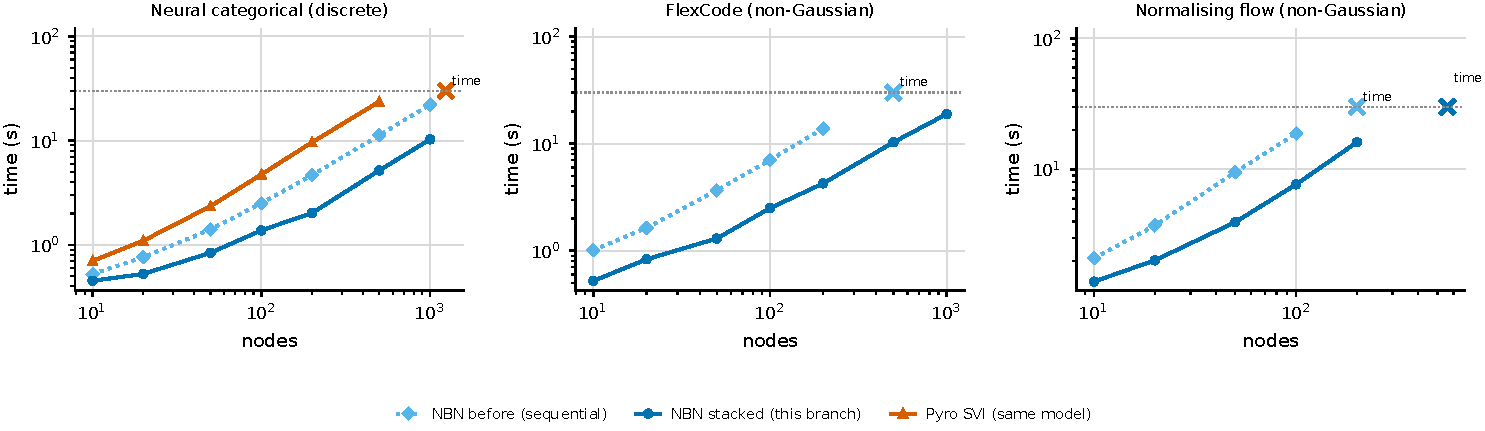
\includegraphics[width=\linewidth]{r2_1_neural_fits.pdf}
\caption{Fit time vs nodes (10 epochs). For the neural categorical, Pyro SVI fits the same model for the same steps.}
\end{figure}
\tabin{r2fit}

\section{Queries on kNN and FlexCode networks (vs previous NBN)}
These queries combine round 1 (barren-node pruning in LW) with round 2 (kNN search, FlexCode
normaliser), so the three versions separate the two effects.
\begin{figure}[H]\centering
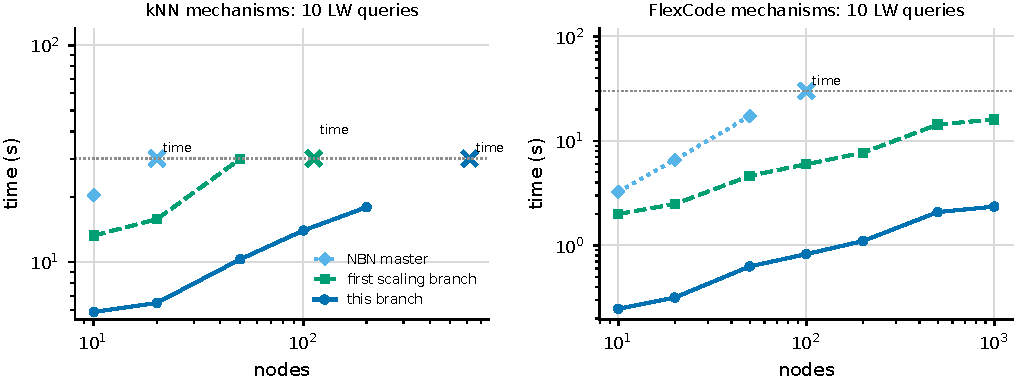
\includegraphics[width=\linewidth]{r2_2_knn_flex_queries.pdf}
\caption{Ten likelihood-weighting queries on networks of kNN (left) or FlexCode (right) mechanisms.}
\end{figure}
\tabin{r2q}
\begin{figure}[H]\centering
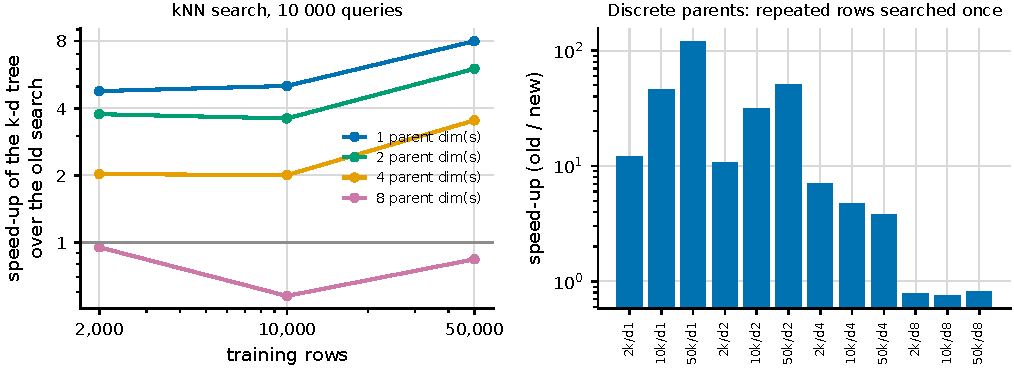
\includegraphics[width=\linewidth]{r2_5_knn_search_micro.pdf}
\caption{kNN search alone. Left: k-d tree vs the old search; at 8 parent dimensions the tree loses, so \code{search="auto"} uses it only up to 4. Right: discrete parents, repeated rows searched once (5, 25, 625 distinct query rows for $d=1,2,4$); at $d=8$ almost all 10\,000 rows are distinct, so the ratio is just the cost of the exact search (about $0.8\times$).}
\end{figure}
\tabin{r2micro}
\tabin{r2flex}

\section{Amortized engines (vs previous NBN)}
\begin{figure}[H]\centering
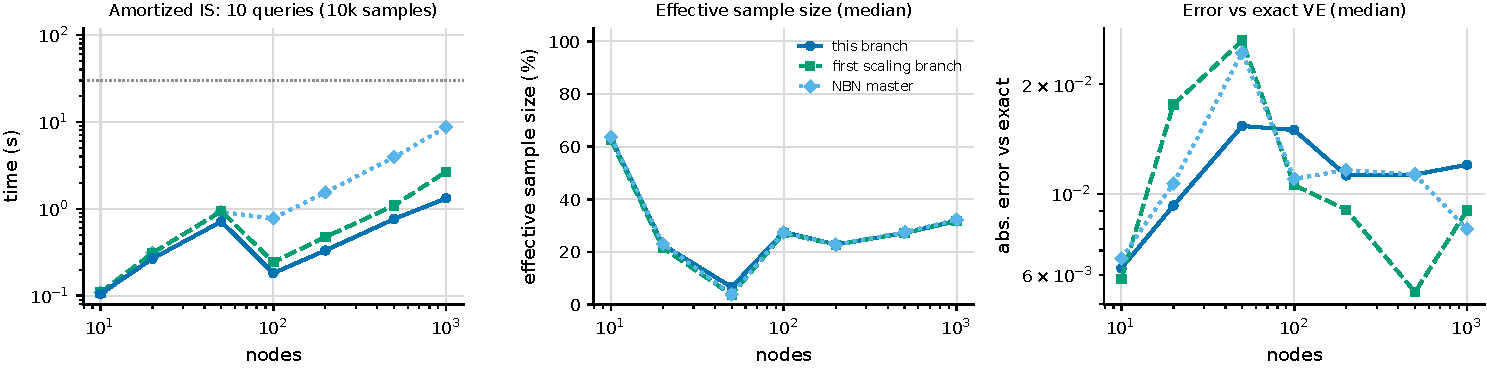
\includegraphics[width=\linewidth]{r2_3_amortized_is.pdf}
\caption{Amortized importance sampling on loose graphs: query time, effective sample size and error against exact VE.}
\end{figure}
\tabin{r2ais}
\tabin{r2aisseeds}
Pruning changes which random numbers are drawn, so single runs differ by Monte Carlo noise (one seed: error 0.012 vs 0.008 at 1000 nodes). Over six seeds the two versions agree: at 1000 nodes mean error $0.0099\pm0.0026$ (this branch) vs $0.0087\pm0.0012$ (master), a difference below one standard error, with the same median ESS/N (0.271); at 200 nodes this branch is lower ($0.015$ vs $0.030$). Same estimator, 3--8$\times$ less time.
\begin{figure}[H]\centering
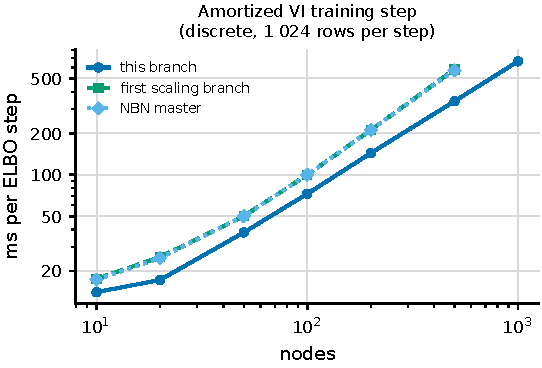
\includegraphics[width=0.55\linewidth]{r2_4_amortized_vi.pdf}
\caption{Amortized variational inference: time per ELBO training step.}
\end{figure}
\tabin{r2avi}

\section{Expert review}
The \code{koller\_claude} expert reviewed the implemented claims against Koller \& Friedman
(printed pages; every reference re-read in the call):
\begin{itemize}
  \item \textbf{Stacked fitting.} Supported by the decomposition of the likelihood under complete
  data and disjoint per-node parameters (Prop.\ 17.1, p.\ 725; the excess risk splits per family,
  Thm 17.3, p.\ 774). Conditions to keep: no shared parameters (§17.5, p.\ 754) and no coupling by
  the optimiser (global-norm clipping, shared schedules); this implementation clips per node and
  uses element-wise Adam. A \emph{shared} held-out split is arguably the cleaner case: the joint
  held-out likelihood is then exactly the sum of the per-node terms (expert's derivation). Caveat:
  for flows, each node keeps the same law of its estimator, but the selection noise of early
  stopping is now common to all nodes (holdout results depend on the split, p.\ 795; small
  validation sets make stopping noisy, p.\ 891). FlexCode's exponent selection already used a
  fixed split, so it is identical to the sequential path.
  \item \textbf{kNN ties.} The book has no instance-based CPD (only the kernel CPD of Box 17.B,
  symmetric in the instances). Lowest-index tie-breaking is reproducible but depends on the row
  order; averaging over all tied neighbours would be order-invariant (possible third option).
  \item \textbf{Certified routing.} Approximation with guaranteed error is NP-hard in general
  (Thms 9.3--9.4, p.\ 291), so the cost of a certified answer must grow somewhere: here like
  $W/P(e)$. The intervals bound inference error for the fitted model, not learning error. When
  memory is the binding constraint, exact \emph{conditioning} (linear space, more time; §9.5,
  pp.\ 315--321) is an alternative to sampling: a candidate for a future router option.
\end{itemize}
Earlier in the round, \code{koller\_claude} and \code{moss\_claude} checked barren pruning under a
learned proposal (same target; asymptotic variance not higher, by a conditional-mean-one and Jensen
argument that neither book states), the ELBO decomposition behind the batched VI loss
(Thm 11.2, p.\ 385; Box 10.A), and the kernel-CPD cost (Box 17.B, pp.\ 730--731).

\section{Limits and notes}
\begin{itemize}
  \item kNN on the GPU (MPS): the exact tie rule costs about 25\% over the old search;
  \code{tie\_break="any"} restores the old speed and behaviour. On CPU the k-d tree is used up to
  4 parent dimensions; beyond that, the exact brute path costs 1.2--1.35$\times$ the old one (micro-benchmark, all sizes). Deduplicating query rows helps only when rows repeat; with almost all rows distinct, it adds nothing and costs little.
  \item Conditional KDE was not changed: its exact cost is $O(N)$ per query, and every faster
  method (tree-based kernel sums) is an approximation (K\&F Box 17.B, pp.\ 730--731).
  \item Amortized VI: the batched path applies only when every node is a plain table CPD; mixed
  networks keep the per-node loop.
  \item Stacked flows: roots (no parents) keep the sequential fit; zero-weight rows in FlexCode
  also keep it.
\end{itemize}

\section*{Reproduce}
\begin{verbatim}
bash benchmarks/scaling/r2.sh          # sweeps: this branch, first branch (v1), master
python benchmarks/scaling/r2_micro.py  # kNN search and FlexCode micro-benchmarks
python benchmarks/scaling/run.py r2_ais --seeds 1 2 3 4 5 --sizes 200 1000 \
    --out benchmarks/scaling/results/r2_ais_seeds.jsonl   # and again with --code <master>
python benchmarks/scaling/r2_analyze.py
cd benchmarks/scaling/report && tectonic -X compile report_r2.tex
\end{verbatim}
\end{document}
